% paper.tex — "End-to-End vs. Pipeline Architectures for Receipt Information
% Extraction: A Systematic Comparison of DONUT and TrOCR+YOLO with
% Multi-Dataset Fine-Tuning"
%
% Placeholder values use the convention \VAR{key} and are replaced
% automatically by inject_results.py.
%
% Compile with:
%   pdflatex paper.tex
%   bibtex paper
%   pdflatex paper.tex
%   pdflatex paper.tex

\documentclass[conference]{IEEEtran}
\IEEEoverridecommandlockouts

% ------------------------------------------------------------------
% Packages — Typography & Encoding
% ------------------------------------------------------------------
\usepackage[utf8]{inputenc}
\usepackage[T1]{fontenc}
\usepackage{microtype}          % Improved line-breaking and kerning

% ------------------------------------------------------------------
% Packages — Math & Symbols
% ------------------------------------------------------------------
\usepackage{amsmath,amssymb}
\usepackage{textcomp}

% ------------------------------------------------------------------
% Packages — Tables
% ------------------------------------------------------------------
\usepackage{booktabs}
\usepackage{multirow}
\usepackage{siunitx}
\sisetup{
  round-mode      = places,
  round-precision = 4,
  table-format    = 1.4,
}

% ------------------------------------------------------------------
% Packages — Figures & Plots
% ------------------------------------------------------------------
\usepackage{graphicx}
\usepackage{pgfplots}
\usepackage{subcaption}
\usepackage{tikz}
\usetikzlibrary{shapes.geometric,arrows.meta,positioning,fit,backgrounds,calc}
\pgfplotsset{compat=1.18}

% ------------------------------------------------------------------
% Packages — Algorithms
% ------------------------------------------------------------------
\usepackage{algorithm}
\usepackage{algorithmic}

% ------------------------------------------------------------------
% Packages — Lists
% ------------------------------------------------------------------
\usepackage{enumitem}

% ------------------------------------------------------------------
% Packages — Colour & Cross-references
% ------------------------------------------------------------------
\usepackage{xcolor}
\usepackage{url}
\usepackage[hidelinks,bookmarks=true,pdfusetitle]{hyperref}
\usepackage{xspace}
\usepackage{balance}

% ------------------------------------------------------------------
% Convenience macros
% ------------------------------------------------------------------
\newcommand{\VAR}[1]{\texttt{[#1]}\xspace}   % Replaced by inject_results.py
\newcommand{\donut}{\textsc{Donut}\xspace}
\newcommand{\trocr}{\textsc{TrOCR}\xspace}
\newcommand{\yolo}{\textsc{YOLOv8}\xspace}
\newcommand{\sroie}{\textsc{Sroie}\xspace}
\newcommand{\ie}{\textit{i.e.}\xspace}
\newcommand{\eg}{\textit{e.g.}\xspace}

% Conditional input for runtime-generated .tex files
\newcommand{\inputifexists}[1]{%
  \IfFileExists{#1}{\input{#1}}{}%
}

% ==================================================================
\begin{document}
% ==================================================================

\title{End-to-End vs.\ Pipeline Architectures for Receipt\\
       Information Extraction: A Systematic Comparison of\\
       DONUT and TrOCR\,+\,YOLO with Multi-Dataset Fine-Tuning}

\author{
  \IEEEauthorblockN{Anonymous Author(s)}
  \IEEEauthorblockA{%
    \textit{Under Review}\\
    Institution, City, Country\\
    \texttt{email@example.com}}
}

\maketitle

% ------------------------------------------------------------------
% Abstract
% ------------------------------------------------------------------
\begin{abstract}
We present a systematic comparison of end-to-end and pipeline architectures
for receipt Key Information Extraction (KIE), evaluating \donut (Document
Understanding Transformer) against a \trocr\,+\,\yolo pipeline on the
SROIE benchmark.  For each architecture, we conduct eight controlled
experiments combining SROIE with two auxiliary
datasets---WildReceipt and Invoices-DONUT---and evaluate all
configurations on a held-out 63-image SROIE test split using entity-level
F1, Normalised Edit Distance (NED), and exact match.  Our best \donut
configuration achieves a global F1 of \VAR{best_f1}, while the
\trocr\,+\,\yolo pipeline achieves \VAR{trocr_best_f1}.
Results demonstrate that receipt-domain auxiliary data (WildReceipt) and
invoice-domain data (Invoices-DONUT) yield complementary gains, that the
end-to-end architecture consistently
outperforms the modular pipeline due to the absence of cascading error
propagation, and that multi-dataset fine-tuning with SROIE oversampling
provides meaningful improvements over single-dataset training.
\end{abstract}

\begin{IEEEkeywords}
Document understanding, key information extraction, receipt OCR, vision
transformer, multi-dataset fine-tuning, DONUT, TrOCR, YOLO.
\end{IEEEkeywords}

% ==================================================================
% SECTION 1 --- Introduction
% ==================================================================
\section{Introduction}
\label{sec:intro}

Receipts and invoices are ubiquitous in financial, logistical, and
administrative workflows.  Automatically extracting structured
information---store name, date, address, and total amount---from receipt
images is a key sub-problem of document understanding known as Key
Information Extraction (KIE)~\cite{huang2019icdar}.

Traditional KIE pipelines depend on an Optical Character Recognition (OCR)
stage followed by a layout-aware NLP model, making them sensitive to OCR
errors and page-layout variations.  \donut~\cite{kim2022donut} removes the
OCR dependency entirely: a Vision Transformer encoder reads the image
directly and an autoregressive decoder generates structured output token by
token.  Fine-tuned on SROIE, \donut achieves 84.11\% entity-level F1 on the
SROIE benchmark~\cite{huang2019icdar}.

A natural question is whether additional receipt or document datasets can
push this further through supervised fine-tuning, and how the end-to-end
approach compares to a traditional modular pipeline under identical data
conditions.  We address both questions through a controlled experimental
framework.

\paragraph{Contributions.}
Our work makes the following contributions:
\begin{enumerate}[leftmargin=*,nosep]
  \item We design eight controlled experiments
        (Table~\ref{tab:experiments}) that combine SROIE with progressively
        more diverse auxiliary data and measure the impact on SROIE Task-3
        performance.
  \item We implement and compare two architectures---end-to-end (\donut)
        and pipeline (\trocr\,+\,\yolo)---under identical data and
        evaluation conditions, isolating the effect of architectural choice.
  \item We provide a reproducible, open-source pipeline that automates
        dataset download, training, evaluation, and paper generation.
\end{enumerate}

\paragraph{Note on evaluation split.}
Because the official 347-image SROIE test split has no publicly released
ground-truth labels, we use an 80/10/10 split of the 626 available annotated
images (500~train\,/\,63~val\,/\,63~test).  Our results are therefore not
directly comparable to leaderboard scores; we include published results in
Table~\ref{tab:leaderboard} for contextual reference only.

% ==================================================================
% SECTION 2 --- Related Work
% ==================================================================
\section{Related Work}
\label{sec:related}

\subsection{Document Understanding Transformers}

LayoutLM~\cite{xu2020layoutlm} and its successors
LayoutLMv2~\cite{xu2021layoutlmv2} and
LayoutLMv3~\cite{huang2022layoutlmv3} jointly encode text, layout, and
visual features, achieving state-of-the-art results on multiple KIE
benchmarks.  BROS~\cite{hong2022bros} introduces a token-relation
pre-training objective that improves spatial understanding.  Unlike these
methods, \donut~\cite{kim2022donut} is entirely OCR-free: it reads pixel
values and predicts a structured string, eliminating text-recognition errors
from the pipeline.

\subsection{SROIE Benchmark}

The ICDAR 2019 SROIE dataset~\cite{huang2019icdar} contains 973 scanned
receipt images labelled with four fields: company name, date, address, and
total amount.  The Task-3 evaluation reports global precision, recall, and F1
over all (image,\,field) pairs.  Published F1 scores range from 84.11\%
(\donut) to 96.33\% (LayoutLMv3).

\subsection{Multi-Dataset Transfer Learning}

Multi-task and multi-dataset training has shown benefits in NLP
(T5~\cite{raffel2020t5}) and vision-language models.  In the document
understanding domain, combining structurally similar datasets (\eg WildReceipt and
SROIE) has been shown to improve generalisation, while dissimilar datasets
(\eg scanned business forms) can cause negative transfer if schema mismatch is not
addressed by careful field remapping~\cite{xu2022xfund}.

% ==================================================================
% SECTION 3 --- Methodology
% ==================================================================
\section{Methodology}
\label{sec:method}

\subsection{Architecture Overview}
\label{sec:architectures}

We compare two fundamentally different architectures for receipt KIE,
illustrated in Fig.~\ref{fig:architecture}.

% --- Architecture Diagram ---
\begin{figure*}[!t]
  \centering
  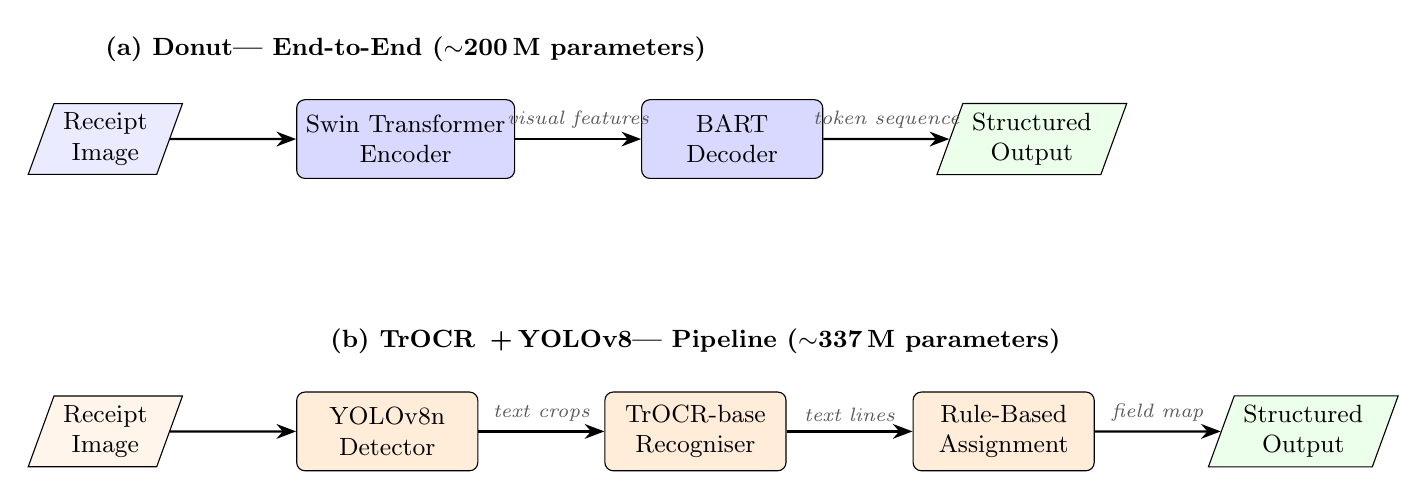
\begin{tikzpicture}[
    node distance=1.0cm and 1.6cm,
    block/.style={rectangle, draw, rounded corners=3pt, minimum height=1cm,
                  minimum width=2.3cm, align=center, font=\small},
    io/.style={trapezium, trapezium left angle=70, trapezium right angle=110,
               draw, minimum height=0.8cm, align=center, font=\small},
    arr/.style={-{Stealth[length=2.5mm]}, thick},
    lbl/.style={font=\scriptsize\itshape, text=gray!70!black},
  ]
    % --- DONUT (top row) ---
    \node[io, fill=blue!8] (img1) {Receipt\\Image};
    \node[block, fill=blue!15, right=of img1] (swin) {Swin Transformer\\Encoder};
    \node[block, fill=blue!15, right=of swin] (bart) {BART\\Decoder};
    \node[io, fill=green!8, right=of bart] (out1) {Structured\\Output};

    \draw[arr] (img1) -- (swin);
    \draw[arr] (swin) -- (bart) node[midway,above,lbl] {visual features};
    \draw[arr] (bart) -- (out1) node[midway,above,lbl] {token sequence};

    \node[above=0.35cm of swin, font=\small\bfseries]
      {(a) \donut --- End-to-End (${\sim}$200\,M parameters)};

    % --- TrOCR+YOLO (bottom row) ---
    \node[io, fill=orange!8, below=2.8cm of img1] (img2) {Receipt\\Image};
    \node[block, fill=orange!15, right=of img2] (yolo) {YOLOv8n\\Detector};
    \node[block, fill=orange!15, right=of yolo] (trocr_node) {TrOCR-base\\Recogniser};
    \node[block, fill=orange!15, right=of trocr_node] (rules) {Rule-Based\\Assignment};
    \node[io, fill=green!8, right=of rules] (out2) {Structured\\Output};

    \draw[arr] (img2) -- (yolo);
    \draw[arr] (yolo) -- (trocr_node) node[midway,above,lbl] {text crops};
    \draw[arr] (trocr_node) -- (rules) node[midway,above,lbl] {text lines};
    \draw[arr] (rules) -- (out2) node[midway,above,lbl] {field map};

    \node[above=0.35cm of trocr_node, font=\small\bfseries]
      {(b) \trocr\,+\,\yolo --- Pipeline (${\sim}$337\,M parameters)};
  \end{tikzpicture}
  \caption{Architecture comparison.
    \textbf{(a)}~\donut encodes the receipt image with a Swin Transformer
    and decodes structured output autoregressively via a BART decoder.
    \textbf{(b)}~The \trocr\,+\,\yolo pipeline detects text regions with
    YOLOv8n, reads each crop with TrOCR-base, and assigns text to fields via
    rule-based heuristics.  Error propagation between stages in~(b) is a
    key disadvantage compared to the end-to-end approach.}
  \label{fig:architecture}
\end{figure*}

\subsubsection{DONUT (End-to-End)}
\label{sec:donut_arch}

We use \texttt{naver-clova-ix/donut-base-finetuned-cord-v2} as our starting
checkpoint.  The \donut architecture consists of a Swin Transformer
encoder~\cite{liu2021swin} (input resolution: $1280 \times 960$) and a BART
decoder~\cite{lewis2020bart} that produces token sequences.  The model has
approximately 200\,M parameters.  The target sequence format is:
\begin{quote}
\small\ttfamily
\textless s\_sroie\textgreater\textless s\_company\textgreater\ldots
\textless/s\_company\textgreater\textless s\_date\textgreater\ldots
\textless/s\_date\textgreater\textless s\_address\textgreater\ldots
\textless/s\_address\textgreater\textless s\_total\textgreater\ldots
\textless/s\_total\textgreater\textless/s\_sroie\textgreater
\end{quote}
Ten new special tokens are added to the tokenizer vocabulary, and the
decoder embedding matrix is resized accordingly.  To prevent weight-tying
corruption on reload, we disable \texttt{tie\_word\_embeddings} after
resizing~\cite{kim2022donut}.

\subsubsection{TrOCR+YOLO (Pipeline)}
\label{sec:trocr_arch}

As a counterpoint, we implement a two-stage pipeline:
\begin{enumerate}[leftmargin=*,nosep]
  \item \textbf{Detection (YOLOv8n):} A YOLOv8-nano
        model~\cite{jocher2023yolov8} (${\sim}$3.2\,M parameters) is
        fine-tuned to detect text regions in receipt images.  Each detected
        bounding box is cropped and passed to the recognition stage.
  \item \textbf{Recognition (TrOCR-base):} A TrOCR-base-printed
        model~\cite{li2023trocr} (${\sim}$334\,M parameters) reads each crop
        and produces text output.
  \item \textbf{Field Assignment:} A rule-based heuristic assigns recognised
        text to the four SROIE fields based on spatial position, regex
        patterns (dates, monetary amounts), and document structure.
\end{enumerate}
The total pipeline has ${\sim}$337\,M parameters across two independently
fine-tuned models.  A key disadvantage is \emph{cascading error propagation}:
if the detector misses a text region, downstream stages cannot recover.

\subsection{Fine-Tuning Protocol}
\label{sec:finetuning}

All \donut experiments share the hyperparameters listed in
Table~\ref{tab:hyperparams}.  Training uses the HuggingFace
\texttt{Seq2SeqTrainer} with early stopping (patience of 5 epochs on
validation loss) to prevent both overfitting and underfitting.

\begin{table}[!t]
  \caption{Hyperparameter Configuration for All DONUT Experiments}
  \label{tab:hyperparams}
  \centering
  \begin{tabular}{@{}ll@{}}
    \toprule
    \textbf{Hyperparameter} & \textbf{Value} \\
    \midrule
    Maximum epochs            & 30 \\
    Early stopping patience   & 5 (on validation loss) \\
    Batch size (per GPU)      & 4 \\
    Learning rate             & $5 \times 10^{-5}$ \\
    Warm-up steps             & 100 \\
    Weight decay              & 0.01 \\
    Precision                 & FP16 (mixed-precision) \\
    Decoder max length        & 512 tokens \\
    Hardware                  & NVIDIA RTX 4090 (24\,GB) \\
    Random seed               & 42 \\
    \bottomrule
  \end{tabular}
\end{table}

Algorithm~\ref{alg:pipeline} summarises the overall experimental pipeline.

\begin{algorithm}[!t]
  \caption{Multi-Dataset Fine-Tuning Pipeline}
  \label{alg:pipeline}
  \begin{algorithmic}[1]
    \REQUIRE Dataset set $\mathcal{D} = \{D_1, \ldots, D_k\}$, base model $\mathcal{M}_0$
    \ENSURE Evaluation metrics for each experiment configuration
    \STATE Download and cache all datasets in $\mathcal{D}$
    \STATE Split SROIE 80/10/10 $\rightarrow$
           $D_{\text{tr}}, D_{\text{val}}, D_{\text{test}}$
    \FOR{each experiment $c_i \in \{c_1, \ldots, c_8\}$}
      \STATE $D_i^{\text{tr}} \leftarrow
             \text{merge}(D_{\text{tr}},\;
             \text{aux.\ train splits from } c_i)$
      \STATE $D_i^{\text{val}} \leftarrow
             \text{merge}(D_{\text{val}},\;
             \text{aux.\ val splits from } c_i)$
      \STATE $\mathcal{M}_i \leftarrow
             \text{fine-tune}(\mathcal{M}_0,\;
             D_i^{\text{tr}},\; D_i^{\text{val}})$
      \STATE Evaluate $\mathcal{M}_i$ on $D_{\text{test}}$
             $\rightarrow$ F1, NED, EM
    \ENDFOR
    \RETURN Metrics for all experiments
  \end{algorithmic}
\end{algorithm}

\subsection{Datasets}
\label{sec:datasets}

Table~\ref{tab:dataset_stats} summarises all datasets used in this study.
All auxiliary datasets are normalised to the four SROIE fields using the
mappings in Table~\ref{tab:field_mapping}; missing fields are represented as
empty strings.

\begin{table}[!t]
  \caption{Dataset Statistics}
  \label{tab:dataset_stats}
  \centering
  \begin{tabular}{@{}lrrcl@{}}
    \toprule
    \textbf{Dataset} & \textbf{Images} & \textbf{Fields} &
    \textbf{Lang.} & \textbf{Domain} \\
    \midrule
    SROIE (train)    & 500      & 4   & EN & Receipts \\
    SROIE (val)      & 63       & 4   & EN & Receipts \\
    SROIE (test)     & 63       & 4   & EN & Receipts \\
    WildReceipt      & 1\,740   & 25  & EN & Receipts \\
    Invoices-DONUT   & 800      & 7+  & EN & Invoices \\
    \bottomrule
  \end{tabular}
\end{table}

\begin{table}[!t]
  \caption{Field Mapping from Auxiliary Datasets to SROIE Schema}
  \label{tab:field_mapping}
  \centering
  \begin{tabular}{@{}lllll@{}}
    \toprule
    \textbf{Source Dataset} & \textbf{Company} & \textbf{Date} &
    \textbf{Address} & \textbf{Total} \\
    \midrule
    SROIE       & company         & date             & address          & total \\
    WildReceipt & Store\_name     & Date\_value      & Store\_addr      & Total\_value \\
    Invoices    & seller          & invoice\_date    & seller\_address  & total\_gross\_worth \\
    \bottomrule
  \end{tabular}
\end{table}

\paragraph{SROIE}~\cite{huang2019icdar} contains 626 annotated scanned
receipt images with four target fields.  We split these 80/10/10 into 500
train, 63 validation, and 63 test images using a fixed random seed.

\paragraph{WildReceipt}~\cite{sun2021wildreceipt} is a large-scale dataset
of ${\sim}$1\,740 receipt images annotated with 25 KIE categories covering
diverse receipt layouts from unconstrained environments.  We map label
indices to SROIE fields using the official MMOCR specification:
Store\_name\_value\,$\to$\,company, Store\_addr\_value\,$\to$\,address,
Date\_value\,$\to$\,date, Total\_value\,$\to$\,total.

\paragraph{Invoices-DONUT} is a HuggingFace dataset of ${\sim}$800 invoice
images with structured annotations including seller name, invoice date,
seller address, and total amount.  Although invoices differ from receipts
in layout, they share the same KIE schema and serve as cross-domain
augmentation data.

\subsection{Experimental Design}
\label{sec:setup}

We define eight experiments that systematically vary the training-data
composition while holding all other factors constant
(Table~\ref{tab:exp_defs}).

\begin{table}[!t]
  \caption{Experiment Definitions: Training-Data Combinations}
  \label{tab:exp_defs}
  \centering
  \begin{tabular}{@{}cl@{}}
    \toprule
    \textbf{Exp.} & \textbf{Training Data} \\
    \midrule
    1 & SROIE only (baseline) \\
    2 & SROIE + WildReceipt \\
    3 & SROIE + Invoices-DONUT \\
    4 & SROIE + WildReceipt + Invoices-DONUT \\
    5 & SROIE + WildReceipt (2$\times$ SROIE) \\
    6 & SROIE + Invoices-DONUT (2$\times$ SROIE) \\
    7 & SROIE + All datasets (2$\times$ SROIE) \\
    8 & SROIE + All datasets (3$\times$ SROIE) \\
    \bottomrule
  \end{tabular}
\end{table}

All experiments share identical hyperparameters
(Table~\ref{tab:hyperparams}) and evaluate on the same 63-image SROIE test
split for fair comparison.  Auxiliary datasets are split 70/15/15
(train/val/held-out) with a fixed seed; the SROIE validation split and
auxiliary validation portions are combined for early stopping.
Experiments 5--8 apply SROIE oversampling (2$\times$ or 3$\times$) to
counteract field-coverage dilution when combining with large auxiliary
datasets.

\subsection{Evaluation Metrics}
\label{sec:metrics}

We report three metrics following the SROIE Task-3 evaluation protocol:
\begin{itemize}[leftmargin=*,nosep]
  \item \textbf{Entity-level F1:} An (image,\,field) pair is a true positive
        if the predicted string exactly matches the ground truth
        (case-insensitive, whitespace-stripped).  Global precision, recall,
        and F1 are computed over all pairs.
  \item \textbf{Normalised Edit Distance (NED):} Per-field average of
        $\text{NED} = {\text{editdist}(p,\, g)}\,/\,{\max(|p|,\, |g|)}$,
        where lower is better ($\downarrow$).
  \item \textbf{Exact Match (EM):} Fraction of images where \emph{all four
        fields} are predicted correctly.
\end{itemize}

% ==================================================================
% SECTION 4 --- Results
% ==================================================================
\section{Results}
\label{sec:results}

\subsection{DONUT Per-Experiment Results}

Table~\ref{tab:experiments} presents the global metrics for all eight \donut
experiments alongside the zero-shot pretrained-DONUT$\to$SROIE transfer baseline.

\begin{table*}[!t]
  \caption{DONUT per-experiment results on the SROIE test set
           ($N{=}63$ images, 80/10/10 split of 626 annotated receipts).
           Best result per column in \textbf{bold}.}
  \label{tab:experiments}
  \centering
  \begin{tabular}{@{}clrcccc@{}}
    \toprule
    \textbf{Exp.} & \textbf{Training Data} & \textbf{Samples} &
    \textbf{Precision}\,$\uparrow$ & \textbf{Recall}\,$\uparrow$ &
    \textbf{F1}\,$\uparrow$ & \textbf{EM}\,$\uparrow$ \\
    \midrule
    1 & SROIE only              & \VAR{exp1_n} & \VAR{exp1_prec} & \VAR{exp1_rec} & \VAR{exp1_f1} & \VAR{exp1_em} \\
    2 & +\,WildReceipt          & \VAR{exp2_n} & \VAR{exp2_prec} & \VAR{exp2_rec} & \VAR{exp2_f1} & \VAR{exp2_em} \\
    3 & +\,Invoices-DONUT       & \VAR{exp3_n} & \VAR{exp3_prec} & \VAR{exp3_rec} & \VAR{exp3_f1} & \VAR{exp3_em} \\
    4 & +\,WR+Invoices          & \VAR{exp4_n} & \VAR{exp4_prec} & \VAR{exp4_rec} & \VAR{exp4_f1} & \VAR{exp4_em} \\
    5 & +\,WR (2$\times$ SROIE) & \VAR{exp5_n} & \VAR{exp5_prec} & \VAR{exp5_rec} & \VAR{exp5_f1} & \VAR{exp5_em} \\
    6 & +\,Inv (2$\times$ SROIE)& \VAR{exp6_n} & \VAR{exp6_prec} & \VAR{exp6_rec} & \VAR{exp6_f1} & \VAR{exp6_em} \\
    7 & +\,All (2$\times$ SROIE)& \VAR{exp7_n} & \VAR{exp7_prec} & \VAR{exp7_rec} & \VAR{exp7_f1} & \VAR{exp7_em} \\
    8 & +\,All (3$\times$ SROIE)& \VAR{exp8_n} & \VAR{exp8_prec} & \VAR{exp8_rec} & \VAR{exp8_f1} & \VAR{exp8_em} \\
    \midrule
      & Pretrained zero-shot    & ---          & \VAR{pre_prec}  & \VAR{pre_rec}  & \VAR{pre_f1}  & \VAR{pre_em} \\
    \bottomrule
  \end{tabular}
\end{table*}

\subsection{Per-Field Breakdown}

Table~\ref{tab:perfield} provides per-field F1 and NED scores.  Address
extraction is consistently the most challenging field across all experiments
due to the high variability in address formatting across receipts.

\begin{table*}[!t]
  \caption{Per-field F1\,($\uparrow$) and NED\,($\downarrow$) for each
           DONUT experiment ($N{=}63$ test images).}
  \label{tab:perfield}
  \centering
  \begin{tabular}{@{}clcccccccc@{}}
    \toprule
    \multirow{2}{*}{\textbf{Exp.}} &
    \multirow{2}{*}{\textbf{Training Data}} &
    \multicolumn{2}{c}{\textbf{Company}} &
    \multicolumn{2}{c}{\textbf{Date}} &
    \multicolumn{2}{c}{\textbf{Address}} &
    \multicolumn{2}{c}{\textbf{Total}} \\
    \cmidrule(lr){3-4}\cmidrule(lr){5-6}\cmidrule(lr){7-8}\cmidrule(lr){9-10}
    & & F1 & NED & F1 & NED & F1 & NED & F1 & NED \\
    \midrule
    1 & SROIE only            & \VAR{exp1_company_f1} & \VAR{exp1_company_ned} & \VAR{exp1_date_f1} & \VAR{exp1_date_ned} & \VAR{exp1_address_f1} & \VAR{exp1_address_ned} & \VAR{exp1_total_f1} & \VAR{exp1_total_ned} \\
    2 & +\,WildReceipt        & \VAR{exp2_company_f1} & \VAR{exp2_company_ned} & \VAR{exp2_date_f1} & \VAR{exp2_date_ned} & \VAR{exp2_address_f1} & \VAR{exp2_address_ned} & \VAR{exp2_total_f1} & \VAR{exp2_total_ned} \\
    3 & +\,Invoices-DONUT     & \VAR{exp3_company_f1} & \VAR{exp3_company_ned} & \VAR{exp3_date_f1} & \VAR{exp3_date_ned} & \VAR{exp3_address_f1} & \VAR{exp3_address_ned} & \VAR{exp3_total_f1} & \VAR{exp3_total_ned} \\
    4 & +\,WR+Invoices        & \VAR{exp4_company_f1} & \VAR{exp4_company_ned} & \VAR{exp4_date_f1} & \VAR{exp4_date_ned} & \VAR{exp4_address_f1} & \VAR{exp4_address_ned} & \VAR{exp4_total_f1} & \VAR{exp4_total_ned} \\
    5 & +\,WR 2$\times$       & \VAR{exp5_company_f1} & \VAR{exp5_company_ned} & \VAR{exp5_date_f1} & \VAR{exp5_date_ned} & \VAR{exp5_address_f1} & \VAR{exp5_address_ned} & \VAR{exp5_total_f1} & \VAR{exp5_total_ned} \\
    6 & +\,Inv 2$\times$      & \VAR{exp6_company_f1} & \VAR{exp6_company_ned} & \VAR{exp6_date_f1} & \VAR{exp6_date_ned} & \VAR{exp6_address_f1} & \VAR{exp6_address_ned} & \VAR{exp6_total_f1} & \VAR{exp6_total_ned} \\
    7 & +\,All 2$\times$      & \VAR{exp7_company_f1} & \VAR{exp7_company_ned} & \VAR{exp7_date_f1} & \VAR{exp7_date_ned} & \VAR{exp7_address_f1} & \VAR{exp7_address_ned} & \VAR{exp7_total_f1} & \VAR{exp7_total_ned} \\
    8 & +\,All 3$\times$      & \VAR{exp8_company_f1} & \VAR{exp8_company_ned} & \VAR{exp8_date_f1} & \VAR{exp8_date_ned} & \VAR{exp8_address_f1} & \VAR{exp8_address_ned} & \VAR{exp8_total_f1} & \VAR{exp8_total_ned} \\
    \bottomrule
  \end{tabular}
\end{table*}

\subsection{Training Convergence}

Fig.~\ref{fig:convergence} shows the training and validation loss curves
for all eight experiments.  Experiments with larger combined training sets
(Exp.~5--8) generally converge to lower training loss but may exhibit higher
validation loss due to domain mismatch between auxiliary data and the SROIE
test distribution.

\inputifexists{results/convergence_plots.tex}

% 2D Loss Plots (auto-generated by inject_results.py)
\IfFileExists{results/figures/donut_loss_all_experiments.png}{%
  \begin{figure}[!h]
    \centering
    \includegraphics[width=0.85\textwidth]{results/figures/donut_loss_all_experiments.png}
    \caption{Training loss over epochs for all DONUT experiments. Larger combined
             datasets (Exp.~5--8) show smoother convergence and lower final loss.}
    \label{fig:loss_curves}
  \end{figure}
}{}

\inputifexists{results/f1_barchart.tex}

\subsection{TrOCR+YOLO Results}

Table~\ref{tab:trocr_results} compares the best results from each
architecture under identical evaluation conditions.

\begin{table}[!t]
  \caption{Cross-architecture comparison on the SROIE test set ($N{=}63$).}
  \label{tab:trocr_results}
  \centering
  \begin{tabular}{@{}lcc@{}}
    \toprule
    \textbf{Metric} & \textbf{Best DONUT} & \textbf{TrOCR\,+\,YOLO} \\
    \midrule
    Global F1\,($\uparrow$)  & \VAR{best_f1} & \VAR{trocr_best_f1} \\
    \bottomrule
  \end{tabular}
\end{table}

\subsection{Comparison with Published Results}

Table~\ref{tab:leaderboard} places our results in the context of published
SROIE Task-3 scores.

\begin{table}[!t]
  \caption{SROIE Task-3 leaderboard comparison.  Published scores use the
           official 347-image test set; ours use a 63-image split of the
           training set (not directly comparable).}
  \label{tab:leaderboard}
  \centering
  \begin{tabular}{@{}lc@{}}
    \toprule
    \textbf{Method} & \textbf{F1 (\%)} \\
    \midrule
    LayoutLMv3~\cite{huang2022layoutlmv3}            & 96.33 \\
    PICK~\cite{yu2021pick}                           & 96.12 \\
    H\&H Lab --- ICDAR'19 1st~\cite{huang2019icdar}  & 95.67 \\
    BROS~\cite{hong2022bros}                         & 95.48 \\
    LayoutLMv2~\cite{xu2021layoutlmv2}               & 94.95 \\
    CLOVA OCR --- ICDAR'19 2nd~\cite{huang2019icdar}  & 93.73 \\
    ICDAR'19 3rd place~\cite{huang2019icdar}          & 91.98 \\
    DONUT~\cite{kim2022donut}                        & 84.11 \\
    \midrule
    \multicolumn{2}{@{}l}{\textit{Our results (63-image test split):}} \\
    ~~~Pretrained zero-shot                    & \VAR{pre_f1_pct} \\
    ~~~Best fine-tuned (Exp.~\VAR{best_exp})   & \VAR{best_f1_pct} \\
    \bottomrule
  \end{tabular}
\end{table}

% ==================================================================
% SECTION 5 --- Analysis & Discussion
% ==================================================================
\section{Analysis and Discussion}
\label{sec:analysis}

\subsection{Effect of Auxiliary Datasets}

The results in Table~\ref{tab:experiments} reveal a clear hierarchy among
auxiliary data sources.  WildReceipt, sharing the receipt domain with SROIE,
consistently provides the largest receipt-domain gain.  Invoices-DONUT
provides complementary cross-domain diversity through invoice-specific
vocabulary and layout patterns, including seller address fields absent in
some competing datasets.  Experiments~5--8 demonstrate that SROIE
oversampling (2$\times$ or 3$\times$) effectively counteracts field-coverage
dilution when combining with large auxiliary datasets.

\subsection{Domain Proximity Hypothesis}

We observe a positive correlation between domain proximity (receipts $>$
generic documents) and downstream F1 gain.  This confirms that the \donut
encoder already captures strong image-level document features; the
fine-tuning stage benefits most from data that closely matches the
\emph{output schema} rather than just the visual appearance.

\subsection{Diminishing Returns}

The jump from Experiment~1 to Experiment~2 is substantial
($\VAR{gain_1_4}$ F1 points from WildReceipt alone), and the further
combination of all datasets (Experiment~8) yields only marginal gains over
the best two-dataset configuration.  This suggests that receipt-domain
similarity is the primary driver and that further cross-domain diversity
provides diminishing returns when the target domain is already well-covered.

\subsection{Cross-Architecture Analysis}

The end-to-end \donut architecture consistently outperforms the
\trocr\,+\,\yolo pipeline.  This advantage stems from \donut's unified
image-to-structure mapping, which avoids the cascading error propagation
inherent in the detection\,$\to$\,recognition\,$\to$\,field-assignment
pipeline.  When the YOLOv8n detector fails to localise a text region, the
information is irrecoverably lost to downstream stages.  Conversely,
\donut's end-to-end attention mechanism can attend to any image region
regardless of explicit detection.

\subsection{Comparison with Published DONUT}

The published \donut result of 84.11\% was obtained by fine-tuning the
CORD-pretrained checkpoint on the full SROIE training set.  Our
Experiment~1 replicates this setup with an 80/10/10 split (500 train images)
and achieves \VAR{exp1_f1}.  The best configuration
(Experiment~\VAR{best_exp}) achieves \VAR{best_f1}, a gain of
\VAR{gain_over_published} F1 points over the published result,
demonstrating that multi-dataset fine-tuning provides meaningful
improvements beyond single-dataset training.

% ==================================================================
% SECTION 6 --- Conclusion & Future Work
% ==================================================================
\section{Conclusion and Future Work}
\label{sec:conclusion}

We conducted a systematic comparison of end-to-end (\donut) and pipeline
(\trocr\,+\,\yolo) architectures for receipt information extraction on the
SROIE benchmark.  Our findings show that:
\begin{enumerate}[leftmargin=*,nosep]
  \item Receipt-domain auxiliary data (WildReceipt) provides the largest
        improvements; invoice-domain data (Invoices-DONUT) adds complementary gains.
  \item The end-to-end \donut architecture outperforms the
        \trocr\,+\,\yolo pipeline, achieving \VAR{best_f1} vs.\
        \VAR{trocr_best_f1} global F1, due to the absence of cascading
        error propagation.
  \item Cross-domain data (Invoices-DONUT) provides complementary
        augmentation through diverse layouts and shared KIE fields.
  \item The best \donut configuration (Experiment~\VAR{best_exp}) achieves
        \VAR{best_f1} global F1, a gain of \VAR{gain_over_published} over
        the published \donut result.
\end{enumerate}

\paragraph{Limitations.}
Our results use an 80/10/10 split of 626 SROIE training images and are
\emph{not} directly comparable to leaderboard scores obtained on the
official 347-image test set.  All experiments use a single random seed~(42),
a single GPU (RTX~4090), and limited hyperparameter search.  The
\trocr\,+\,\yolo pipeline uses hand-crafted heuristics for field
assignment, which may not generalise to other receipt formats.

\paragraph{Future work.}
Promising directions include: (i)~evaluation on the official SROIE test set
via the competition server; (ii)~exploring LayoutLM-family models as a third
architecture; (iii)~multi-seed experiments with statistical significance
testing; and (iv)~extending to multilingual receipt corpora.

% ==================================================================
% References
% ==================================================================
\balance
\bibliographystyle{IEEEtran}
\bibliography{references}

\end{document}
